\chapter{Introduction} % (fold)
\label{cha:introduction}
Before the computer mathematical computations were done by hand which was a tiresome and error-prone process.
In modern times computers have become the main target for doing extensive computations, and their \acrfullpl{cpu} are what the majority of programming languages apply to.
The \acrshort{cpu} architecture is designed to efficiently handle sequential instructions and modern compilers, such as the Intel C++ compiler, can even exploit the \acrshortpl{cpu}  advanced instructions, such as \acrfull{simd}, in order to speedup certain workloads, such as doing similar operations on more data for example scaling every element in an array by a constant factor. \citep{INTEL_SIMD}
As applications and computations grow larger and more complex, programmers and mathematicians find themselves in need of more and more computation power. \citep[pp. 4]{OpenCL_AMD}
At the moment this demand is met with faster multi-cored \acrshortpl{cpu} however Moore's law, which predicts an exponential growth in transistor count in and integrated circuit thus resulting in faster computations on said \acrshortpl{cpu}, might come to an end.
A former engineer from Intel foresees this stagnation of Moore's Law as soon as 2020 or 2022; hence alternatives to using the \acrshort{cpu} architecture needs to be explored.\citep{Moore2013}

One of these options is the \acrfull{gpu}, which mainly is used to generate the graphics that are displayed on the screen.
The \acrshort{gpu} is specialised in performing a vast number of smaller computations in parallel.
Because of this specialisation, the \acrshort{gpu} can handle data parallel workloads just as the \acrshort{cpu} can handle task parallel workloads.
Mathematicians and programmers alike can utilise this advantage and hereby complete compute intensive computations on big sets of data in parallel with better performance than on a \acrshort{cpu}, assuming these computations can be executed in parallel.
The concept of executing computations on the \acrshort{gpu} not related to graphics, is commonly know as \acrfull{gpgpu}.

In recent years this concept has gained increasingly popularity amongst a wide range of different subjects, which requires some form of computation.
Dr. Ian Lane at Carnegie Mellon University have used this to his advantage, in his research on speech and language processing, significantly increasing the performance at which his system, Hydra, can transcript speech. \citep{NvidiaSpotlightIan}
The power provided by the \acrshort{gpu}, is also used in fields where simulations and predictions are the primary focus. 
Bill Putman, a NASA research meteorologist in Global Modelling and Assimilation Office, and his team restructured one of their modelling tools to take advantage of the \acrshortpl{gpu} performance. \citep{NvidiaSpotlightNasa}
Many other areas of research could benefit from the use of \acrshort{gpgpu}.

This relatively newfound interest for using the \acrshort{gpu}, as it has become increasingly difficult to improve the \acrshort{cpu}.
For the past few years, the average Intel \acrshort{cpu} has not increased significantly in regards to clock speed, most are about 3.7GHz.
Even the highest clock speeds, seem to not be improving beyond 9GHz however these clock-speeds produce so much heat, that they require liquid nitrogen for cooling.
Aside from the prediction that Moore's Law will end, another observation of processor development is also no longer available, the Dennard scaling.
This states that the power density required to run a of transistor of a given size will stay constant; thus scaling down the power used, as the transistor fell in size, e.g. scaling down the transistor's linear size by 2, would scale down its power by 4 halving both voltage and current.\citep{DennardScaling}
The reason for this no longer being valid, is the fact that the transistor gates are so thin it affects their structural integrity, and currents stat to leak.\citep{CPUClockSpeeds}
These problems give reason to search for other ways of increasing computational speeds, such as looking to the \acrshort{gpu}.


\begin{itemize}
	\item How do \acrshortpl{gpu} do parallel calculations, and why and when is it better at it than the \acrshort{cpu}?
	\item How can one utilise the functionality found in the \acrshort{gpu} for a given field, without an extensive knowledge of processor architecture?
	\item What factors must be considered when using the \acrshort{gpu} rather than the \acrshort{cpu}? 
\end{itemize}

The following sections will go into further detail regarding both the hard- and software used to achieve the performance the \acrshort{gpu} offers.
Furthermore it will be described how one can utilise the \acrshort{gpu} for its increased computing power, and the different opportunities for doing so. 

\newpage
% chapter introduction (end)

\section{Computation architectures}
\label{sec:comparch}
Computations are often performed on a computer's  \acrshort{cpu}.
A \acrshort{cpu} is often fastest for calculations and task not requiring immense computing power, as well as any calculation not parallelisable.
The \acrshort{cpu} consists of only a few cores which are very fast at performing sequential serial processing. \citep{whatisgpu}
In recent years developers and scientists seem to have developed an interest for performing calculations on Dedicated Graphic Processing Units. \citep{gpurise}
This is a different architecture which was intended for graphics processing.
It seems that the \acrshort{gpu} can be utilised for General-Purpose computing for some computational problems, with a performance improvement over a \acrshort{cpu}.
In the following text we explore the possibilities that a \acrshort{gpu} architecture offers.
\todo{Vi har lige skrevet det her i indledningen ? Skal det med igen ? Eller slet ? - Søren}

\acrshort{gpu}s are commonly used in both private and professional environments, for games and accelerating graphic intensive programs such as Adobe Photoshop and 3D rendering tools. \citep{NVIDIAADOBE,STEAMHW}
The \acrshortpl{gpu} architecture can also be used advantageously for certain types of computations, primarily computations which can be done in parallel. 
An example of this can be calculating different properties of the pixels on a screen. 
The screen can then be divided into different sections called blocks and the computations for each block of data is divided internally on the \acrshort{gpu} to its threads.
This is possible because the specific calculations do not require results from the other calculations, i.e. they are parallelisable.
Unlike the cores in the \acrshort{cpu}; the cores in the \acrshort{gpu} are not designed to perform sequential serial processing, instead its cores are designed to handle multiple tasks at once. 
As such running sequential code on the \acrshort{cpu} will run faster, whereas more compute-intensive functions may be better suited for the \acrshort{gpu}, given the computations can be parallelised. \citep{NvidiaGPGPU}
The aforementioned example with pixels can be viewed as a matrix being divided into blocks, so the same method of parallelised workflow can be applied. 
For linear algebra, there are especially many operations on matrices where the problem can be split to independent subproblems.

\begin{figure}[h!]
\centering
 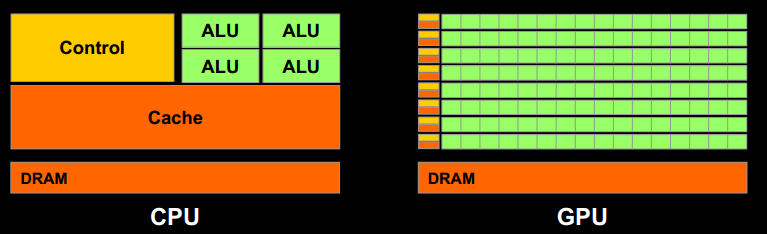
\includegraphics[width=1\textwidth]{figures/GPUCPUimage.png} % trim=4.85cm 15cm 0.85cm 1cm
\caption{A basic representation of the Transistor allocation on a \acrshort{gpu} compared to a \acrshort{cpu}. \citep{NvidiaCUDASeminar}}\label{image:gpucpuimage}
\vspace{-15pt}
\end{figure}

A simple representational comparison of a \acrshort{cpu}'s --- and a \acrshort{gpu}'s transistor usage is shown in \myref{image:gpucpuimage}.
The \acrshort{gpu} consists of many less powerful cores where the \acrshort{cpu} consists of a few more powerful ones, the greater amount of cores allows for more computational power.
But to be able to utilise this computation power a problem must able to be split up, so many or all the cores in the \acrshort{gpu} is used.
As of Q1 2015 an example of a modern high end desktop \acrshort{cpu} is the Intel Haswell core i7 5960X which has 8 cores. \citep{puget}
A contemporary high end \acrshort{gpu} is the NVIDIA GTX 980 which has 2048 CUDA cores. \citep{techpowerup,gtx980}
Due to their architectural differences the \acrshort{gpu} allows for about 12 times more operations per second.\todo{Vi kan sætte en fodnote ind med de beregninger der var her tidligere evt :P ? - Søren}

This makes the \acrshort{gpu} particularly useful for large and complex computations if it is possible to distribute the workload among the \acrshort{gpu}'s cores.
However, the \acrshort{gpu} has an overhead cost.
This means that moving data and computations to the \acrshort{gpu} is time consuming.
Therefore the computation must be of a certain size, before the advantage of parallel \acrshort{gpu} computations exceeds the cost of transferring calculations onto the \acrshort{gpu}.
To illustrate this problem as well as finding an approximate computation size where the \acrshort{gpu} is advantageous some test problems have been written. 
These problems perform different operations on all elements in a matrix. 

\subsection{\acrshort{gpu} and \acrshort{cpu} computations comparison}\label{sub:gpubechmark}
To compare the computational speed of a \acrshort{gpu} and a \acrshort{cpu} for operations on each element in a matrix we have written two programs.
A program written in regular C targeting the \acrshort{cpu} and an equivalent program written in C with CUDA libraries targeting the \acrshort{gpu} for computations.
\todo{Skal der ikke stå noget om hvad CUDA er her ??}
Further explanation of this test and the full source code of both programs and the accompanying scripts can be found in \myref{app:gpuoverhead} and \myref{app:cd}.

Both programs have been run with multiple sizes of the matrix.
The execution times for the two have been compared to find an estimated threshold for when the \acrshort{gpu} power overtakes the data transfer.
The test case for the following comparison consists of seven operations on a square matrix of size n.
As an example, with a square matrix of size $n$ as input the amount of calculations is $7*n^2 = O(n^2)$ operations. 
And there are $n^2 = O(n^2)$ numbers in the matrix which will be operated on.
The operations are division, multiplication, addition and subtraction.
The result can be seen on \myref{image:benchmark}.
\begin{figure}[h!]
\centering
 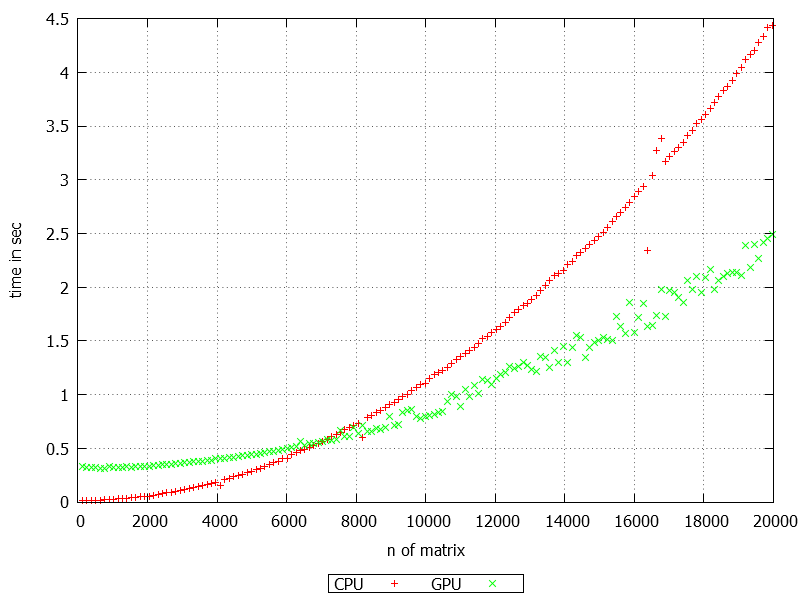
\includegraphics[width=1\textwidth]{figures/benchmark.png} % trim=4.85cm 15cm 0.85cm 1cm
\caption{A benchmark of performing seven operations on each element in a square matrix with size n on a \acrshort{cpu} and a \acrshort{gpu} respectively.}\label{image:benchmark}
\vspace{-15pt}
\end{figure}

The results show that in this case the \acrshort{gpu} becomes advantageous when n reaches about 7000 as can be seen in \myref{image:benchmark}
When n is 7000 the size of the matrix represent operations on almost 50 millions elements.
<<<<<<< HEAD
This is a large amount of data but this is partly due to the simple operations done on the elements in the matrix, we believe that the threshold would happen earlier for a more computation heavy calculation on the elements in the matrix.
=======
This is a large amount of data but this is partly due to the simple operations done on the elements in the matrix, we believe that the threshold would happen earlier for more complex operations on the elements in matrix.\todo{og hvorfra ved vi at det er fordi det er simple operationer? og hvorfor mener vi thresholden ændres med andre operationer?}
>>>>>>> master
In addition to the threshold, the result also confirms that as the dataset grows the \acrshort{gpu} becomes exponentially more useful for computing the data fast.
 %label sec:comparch
\section{Existing solutions} % (fold)
\label{sec:state_of_the_art}
In this section different approaches to \acrshort{gpgpu} using existing programming languages and libraries will be presented.
Each language and library will be running with either the OpenCL or the CUDA framework.
Every language and library described in this section can be found on \myref{tbl:sota} for an overview of their comparisons.
      
\subsection{Libraries} 
There exists libraries for programming languages in order to utilise the \acrshort{gpu} for computations by binding either to OpenCL or CUDA.
Generally the libraries used for \acrshort{gpu} work often requires a lot of boilerplate and has what we deem to be a low level of abstraction.
The level of abstraction is based on how much control the programmer of the code has of the computer's resources.
I.e. if the programmer needs a line of code to allocate memory for each of the computations in the code, that results in low abstraction.
Boilerplate is the pieces of code which will have to be written with little to no alteration, in many different places of the code.
An example could be when making a call to a \acrshort{gpu}, the boilerplate might be the code which handles this communication.
As an example we will look at C, Java and R, and some of their \acrshort{gpu} Libraries.
Jcuda is a library for Java which support the use of CUDA, it has a lot of boilerplate, and low/medium abstraction level. \citep{Java_library}
Jcuda requires many imports and the user needs to allocate a memory block for each element which causes the boilerplate code and the level of abstraction given. \citep{Java_malloc}
C has libraries such as CUDA C, OpenCL C and others.
These C libraries have the same problem as with the Java library as one needs to allocate memory for almost everything, and there is a lot of redundancy which creates a lot of boilerplate.
The abstraction level is therefore deemed low as one must keep in mind what is where and what can be done with each specific element. \citep{C_CUDA} 
There is also different libraries for the R language, one of which is called rpud.
It provides many functions from the R language, which can be performed on the \acrshort{gpu}, and it is based on CUDA.
We deem that it has a high level of abstractions, since it is just function calls, without any memory allocation or direct \acrshort{gpu} calls from the source code. \citep{Rcuda} 

\subsection{Theano (Python)}
Theano is a Python library that allows one to define, optimise, and evaluate mathematical expressions involving multi-dimensional arrays, while utilising the \acrshort{gpu}.
The library has two ways of using the \acrshort{gpu}; one with CUDA as back-end, and the other that should support any OpenCL compatible device as well NVIDIA cards.
The OpenCL implementation however does not support all the options available in the library due to an incomplete port of an old back-end.
While Theano supports CUDA and OpenCL, there is quite a bit of boilerplate and one must write different code in order to use either.	
The scoping rules for Python which Theano uses are quite special where the compiler looks for a variable in four different scopes.
These scoping rules seems to be exclusive to the Python language.
This can cause some problems for new programmers of the language, because these scoping rules are special.
 Theano does not require that the programmer allocates memory for arrays.
We deem that Theano has a medium level of abstraction since one has to declare if the \acrshort{gpu} should be used and can only operate on single precision floats of 32 bits.
But on the other hand Theano does optimise the code by replacing methods with a \acrshort{gpu} versions of the same methods to create transparency. \citep{Theano,Theano_GPU,bergstratheano, LEGB}

\subsection{MATLAB}
MATLAB is a high-level mathematical programming language with an interactive environment.
MATLAB supports the use of parallel computations in the form of using either a \acrshort{gpu} or cloud computing.
It only natively supports the use of CUDA enabled NVIDIA \acrshortpl{gpu} for its parallel computations on \acrshortpl{gpu}, but OpenCL extensions do exist such that it becomes possible to use other devices.
MATLAB uses static scoping  with rules very similar to programming languages like.
The user of MATLAB much declare when the \acrshort{gpu} must be used and also allocate memory for these tasks.
Declaring the memory gives a lot of boilerplate since it needs to be done for each element that one wants to compute. \citep{MATLAB_backend,MATLAB_benchmark}

Using the interactive environment provided by MATLAB there are built in tools for parallel computations on \acrshortpl{gpu}.
These tools provide a higher level of abstraction such as parallel for-loops (parfor) and special array types for distributed processing.
For \acrshort{gpu} computing MATLAB simplify parallel code development by abstracting away the complexity of managing computations and data. \citep{MATLAB_parallel}

\subsection{Julia}
Julia is a high-level, high-performance dynamic programming language for technical computing, with syntax familiar to users of other technical computing environments.
Julia is designed for parallelism and cloud computing; making it efficient and easy to use for these tasks.
Julia has a high level of abstraction because the user only needs a single keyword (\@parallel) for it to do the calculation in parallel.
The code is therefore looking clean without any boilerplate and is easy to read.
Julia uses both OpenCL and CUDA as back-end making it very compatible and easy to use on different systems and devices.
Julia uses similar scoping rules as MATLAB.\citep{Julia_Git, Julia_scope,Julia}

\begin{table}
	\centering
    \colorlet{shadecolor}{gray!40}
    \rowcolors{1}{white}{shadecolor}
	\begin{tabular}{|l|c|c|l|l|}
	\hline
	\textbf{Language} & \textbf{CUDA}         & \textbf{OpenCL} & \textbf{Abstraction} & \textbf{Comment}			  		\\ \hline
	Theano   & \cmark           & \cmark            & High      &  Native                                                          \\ \hline
	Matlab   & \cmark           & \cmark            & Low/High        &  OpenCL via extensions, CUDA is native                                                         \\ \hline
	Julia    & \cmark           & \cmark              & High        &  Both via extensions                                                          \\ \hline
	R        & \cmark           & \cmark            & Low/High    & Abstraction is depended on the use of either CUDA or OpenCL \\ \hline
	C   & \cmark           & \cmark            & Low         & via CUDA C, and OpenCL C (Both are supersets of C)                                           \\ \hline
	Java     & \cmark           & \cmark              &   Low          & Bindings such as jcuda and jocl                                            \\ \hline
	\end{tabular}
	\caption{Existing GPU supporting languages. }\label{tbl:sota}
\end{table}
                

\subsection{Conclusion}  

The different languages mentioned in this section all have some way of communicating with the \acrshort{gpu} using both CUDA and OpenCL, which also can be seen on \myref{tbl:sota}.
They all require the user to specify when to use the \acrshort{gpu} instead of the CPU, and the level of abstraction varies, where some require a lot of control of the programmer, and others require specific function calls to \acrshort{gpu} functions.

This explicit processor targeting seems inconvenient, and it takes away focus from the calculations done in the program.
On the other hand, it gives the programmer more control of where the code is executed.
This aspect requires a deeper knowledge of processor architecture, and we deem that greater abstraction is more important than the control of processor targeting.

They are all usable for general purpose programming, except the libraries for R, which only provides the programmer with specific R functions to be computed on the \acrshort{gpu}.
For scientific computing, especially oriented towards matrices and vector calculations such as linear algebra uses, these are all viable options.

The control of memory on the CPU and the \acrshort{gpu} is different, so allocating memory is more difficult when you transfer the calculations to the \acrshort{gpu}.
Therefore languages that require the programmer to allocate memory themselves, takes away focus from the computations that need to be done.
We deem that allocating memory for arrays and matrices is unnecessary.
                     
\newpage
\section{Problem statement}
\label{sec:problem}

\myref{subsec:gputest} shows that calculations on matrices, when sufficiently large, can take a long time to compute sequentially. 
Therefore it is smarter to parallelise these computations, and even better to do so on a \acrshort{gpu} compared to a \acrshort{cpu}, due to its internal architecture.
Many linear algebra calculations can be parallelised since it often contains large datasets where operations on the data does not depend on previous calculations.
An example of this could be matrix calculations where most operations can be split into independent sub calculations.
Therefore the computation time of these calculations can be significantly improved using the parallel computing capabilities on the \acrshort{gpu}, given the matrices are of sufficient size.

Writing programs which can be run on a \acrshort{gpu}, can be time consuming using the languages found in \myref{sec:state_of_the_art}.
It is time consuming due to the difficulty of writing code in some of these languages like OpenCL C, and CUDA C.
Therefore we believe that more abstraction and less boilerplate when writing code to the \acrshort{gpu} would serve well and reduce the workload on the people programming for the \acrshort{gpu}.
In the rest of this paper, the following problem will be thoroughly investigated, not only in the design of the syntax and the semantics of the language, but also in the design of the compiler.\todo{Vi beslutter os allerede her for at lave en compiler? Skal vi ikke fjerne det og ændre det til noget med "the design of translating the code" eller noget? -Søren}

\[
  \left[
  \begin{minipage}{\textwidth}
  \centering
  \begin{minipage}{0.96\textwidth}
  How does one design a programming language, with a corresponding compiler, which compiles source code to execute on the \acrshort{gpu} at runtime for certain linear algebra calculations, such as matrix operations?
  %%How does one design a programming language, with a corresponding compiler, for technical computing that is capable of performing common operations of linear algebra, while targeting \acrshort{gpu}s as execution platform?
  
  %%Alternative%%
  %%How do you design a programming language and a compiler for this language, which is able to compute parallel linear algebra calculations using the \acrshort{gpu} instead of the CPU without the programmer specifying so?
  
  %%How would a programming language and a compiler be programmed for a language specific for computing paralles linear algebra calculations using the \acrshort{gpu} instead of the CPU without the programmer choosing so specifically.  

  %%Is it possible to design a programming language for numerical computation with a focus on matrices, which is simple to use but also fast by taking advantage of the \acrshort{gpu} on modern computers? How would such a language be implemented? 

  %%How can a simple programming language, which compiles code targeting the \acrshort{gpu}, be construed so it's easier to perform matrix calculations? 

  %%Is it possible to construct a programming language in which matrix operations and linear algebra can be performed, with the power of the \acrshort{gpu}, without the programmer having to worry about boilerplate code. 
  \end{minipage}
  \end{minipage}
    \right]
\]